\documentclass[10pt]{article}
\usepackage{fullpage}
\usepackage{setspace}
\usepackage{parskip}
\usepackage{titlesec}
\usepackage[section]{placeins}
\usepackage{xcolor}
\usepackage{breakcites}
\usepackage{lineno}
\usepackage{hyphenat}





\PassOptionsToPackage{hyphens}{url}
\usepackage[colorlinks = true,
            linkcolor = blue,
            urlcolor  = blue,
            citecolor = blue,
            anchorcolor = blue]{hyperref}
\usepackage{etoolbox}
% \makeatletter
% \patchcmd\@combinedblfloats{\box\@outputbox}{\unvbox\@outputbox}{}{%
%   \errmessage{\noexpand\@combinedblfloats could not be patched}%
% }%
\makeatother


\usepackage{natbib}




\renewenvironment{abstract}
  {{\bfseries\noindent{\abstractname}\par\nobreak}\footnotesize}
  {\bigskip}

\titlespacing{\section}{0pt}{*3}{*1}
\titlespacing{\subsection}{0pt}{*2}{*0.5}
\titlespacing{\subsubsection}{0pt}{*1.5}{0pt}


\usepackage{authblk}


\usepackage{graphicx}
\usepackage[space]{grffile}
\usepackage{latexsym}
\usepackage{textcomp}
\usepackage{longtable}
\usepackage{tabulary}
\usepackage{colortbl}
\usepackage{wrapfig}
\usepackage{booktabs,array,multirow}
\usepackage{amsfonts,amsmath,amssymb}
\providecommand\citet{\cite}
\providecommand\citep{\cite}
\providecommand\citealt{\cite}
% You can conditionalize code for latexml or normal latex using this.
\newif\iflatexml\latexmlfalse
\providecommand{\tightlist}{\setlength{\itemsep}{0pt}\setlength{\parskip}{0pt}}%
\AtBeginDocument{\DeclareGraphicsExtensions{.pdf,.PDF,.eps,.EPS,.png,.PNG,.tif,.TIF,.jpg,.JPG,.jpeg,.JPEG}}
\usepackage[utf8]{inputenc}
\usepackage[ngerman,greek,english]{babel}
\usepackage{float}






% Edit this header.tex file to include frontmatter definitions and global macros

% Add here any LaTeX packages you would like to load in all document blocks
% \usepackage{xspace}

% Add here any LaTeX macros you would like to load in all document blocks
% \def\example{This is an example macro.}

% -----

\iflatexml
% Add here any LaTeXML-specific commands

% -----

\else
% Add here any export style-specific LaTeX commands. These will only be loaded upon document export. 
% \paperfield{Subject domain of my document}
% \keywords{keyword1, keyword2}
% \corraddress{Author One PhD, Department, Institution, City, State or Province, Postal Code, Country}
% \fundinginfo{Funder One, Funder One Department, Grant/Award Number: 123456.}
\fi


\begin{document}

\title{UV Index assessment and trend analysis from hourly 
measurements during twenty years (2000-2019) over the Mexico City Metropolitan Area}


\author[1]{Adriana Ipiña}%
\author[2]{Gamaliel López-Padilla}%
\author[1]{Rubén D Piacentini}%
\author[3]{Sasha Madronich}
\affil[1]{Instituto de Física Rosario (CONICET-UNR), Rosario, Argentina}%
\affil[2]{Facultad de Ciencias Físico Matemáticas, Universidad Autónoma de Nuevo León, San Nicolás de los Garza, México}%
\affil[3]{National Center for Atmospheric Research, Boulder, Colorado USA}%ario }%


\vspace{-1em}



  \date{\today}


\begingroup
\let\center\flushleft
\let\endcenter\endflushleft
\maketitle
\endgroup





\selectlanguage{english}
\begin{abstract}
The UV Index is a measure of the risk of suffering erythema from
short-term solar exposure. Mexico City is one of the most populated
cities in the world, and could experience large exposures due to its
location at 2240 m above sea level, and its intertropical latitude. In
the present study~we analyzed around 2 million ground-based UV Index
measurements from the Secretariat of the Environment of the Mexico City
Government during two decades (2000-2019) over the Mexico City
Metropolitan Area. An increasing trend in the UV Index, of 0.66 \% per
year was found. Trends in criteria pollutants PM\textsubscript{10}, CO,
NO\textsubscript{2}, O\textsubscript{3} and in
AOD\textsubscript{340}~were also estimated. The monthly mean UV Index
value at solar noon reaches barely 10.5 under all sky conditions, along
the year.~UV Index data derived from OMI-Aura/NIVR-FMI-NASA measurements
of ozone and clouds ranged between 6.4 and 14.9. The maximum UV Index
from satellite data as well as the highest~UV Index~ground-based values
were similar, both in Extreme qualification range of WHO (World Health
Organization). The UV Index was used to estimate the Standard Erythema
Dose (SED) per hour for high sun under clear sky conditions, and from
these we estimate exposure times as a limit to avoid sunburn for typical
skin phototypes in Mexico City.~These results contribute to exhaustive
knowledge of UV Index in a highly populated region. This assessment
based on climatology can be of interest for applications in the use of
solar energy, validation of radiative transfer models, study of
influence of pollutants as well as preventive public health campaigns.%
\end{abstract}%



\sloppy


\emph{Keywords: UV~Index, Climatology, Ground-based measurements,
Satellite data, Standard Erythema Dose\emph{.~}~}


\section*{Introduction}

{\label{874460}}

Mexico City is the largest city in North America by number of
inhabitants and one of the largest urban agglomeration in the
world~\hyperref[csl:1]{(UN, 2014)}. The latitude and longitude coordinates for the
city are 19.4\selectlanguage{ngerman}°N and 99.1°W, at an average height of 2240 meters above
sea level. The Mexico City Metropolitan Area (MCMA) is surrounded by
mountain ridges exceeding 5000 m asl and has been the subject of
multiples studies related to air quality due to intense anthropogenic
activity~\hyperref[csl:2]{(Doran et al., 1998}; \hyperref[csl:3]{Molina et al., 2007}; \hyperref[csl:4]{Molina et al., 2010}; \hyperref[csl:5]{Tzompa-Sosa et al., 2017)}. The complex topography and thermal
inversions inhibit winds that sweep away pollution and influence the
surface energy balance~\hyperref[csl:6]{(Whiteman et al., 2000}; \hyperref[csl:7]{Tejeda-Martínez and Jáuregui-Ostos, 2005}; \hyperref[csl:8]{Zhang et al., 2009)}. Solar radiation varies along
the hours of the day and the days of the year, as well as via its
dependence of atmospheric components that attenuate the different
wavelengths. The ultraviolet (UV) range is only a small part of total
incident irradiance, but plays a key role in atmospheric
photochemistry~\hyperref[csl:9]{(Leighton, 1961}; \hyperref[csl:10]{Seinfeld and Pandis, 2016)}. On the pathway through the
atmosphere, photons experience scattering by air molecules, aerosol
particles (haze) and clouds, as well as absorption by gases such as
ozone (O\textsubscript{3}) and nitrogen dioxide (NO\textsubscript{2}),
and some aerosols. An increase in ozone concentration in polluted
boundary layers is also generated by strong UV photon fluxes interacting
with anthropogenic precursor emissions~\hyperref[csl:9]{(Leighton, 1961}; \hyperref[csl:11]{Finlayson-Pitts and Pitts, 2000)}. Conversely,
aerosols may increase or reduce the insolation and photolysis rates, and
thus affect photochemical smog formation~\hyperref[csl:12]{(Dickerson, 1997)}. A
modelization of~actinic flux applied to Mexico City, showed a decrease
at the surface and an increase aloft, mainly due to the presence of
aerosols~\hyperref[csl:13]{(Palancar et al., 2013)}. Likewise, a reduction in the~ measured and
theoretical values of nitrogen dioxide photolysis rate was attributed to
attenuation of spectral actinic solar flux by
aerosols~\hyperref[csl:14]{(Castro et al., 2001)}.~

Despite multiple efforts to monitor and characterize air quality in the
Mexico City basin, few studies have specially focused on global solar
radiation~\hyperref[csl:15]{(Galindo et al., 1991}; \hyperref[csl:16]{Qui{\~{n}}ones and Almanza, 2014}; \hyperref[csl:17]{Matsumoto et al., 2014)}. In the mid-1990s, two studies about UV
solar irradiance measurements in the Mexican Valley, for periods shorter
than 3 years, were published. One of these studies suggested~a
significant attenuation on UV intensity due to tropospheric ozone,
comparing measurements in downtown and outskirts of the Mexico
City~\hyperref[csl:18]{(Acosta and Evans, 2000)}. Another study reported that Mexico City had
lower ultraviolet fluxes (around 25\% at noon and 50\% in the afternoon)
compared to Colima, a city placed at the same latitude, lower elevation
(ca. 300-500 m asl) and almost pollution-free.~\hyperref[csl:19]{(Galindo et al., 1995)}. To
our knowledge, these are the only published long-term measurements of UV
radiation in Mexico City. Short-term measurements and comparisons with
radiative models were reported by~\hyperref[csl:13]{(Palancar et al., 2013)}. Other UV
measurements have been carried out to estimate aerosol optical
properties at UV wavelengths, e.g. using UV Multi-Filter Rotating
Shadowband Radiometers (MFRSRs) to estimate aerosol single scattering
albedo~\hyperref[csl:20]{(Goering, 2005}; \hyperref[csl:21]{Corr et al., 2009)}, but did not focus on the UV Index. ~

UV Index (UVI) is an indicator related to the intensity of the solar UV
radiation at the Earth's surface and~the risk for persons to suffer
sunburn,~and may be relevant to chronic effects due to prolonged
exposure, such as skin cancer. Fitzpatrick classification defines six
phototypes (I-VI) or skin colors from pale to dark, correlated to the UV
radiation sensitivity~\hyperref[csl:22]{(Fitzpatrick, 1974)}. The International Commission
on Illumination (CIE) established an action spectrum for erythema (or
erythemal sensitivity) of human skin~using phototype II~from Fitzpatrick
classification~\hyperref[csl:23]{(CIE, 2014)}. According to the World Health
Organization (WHO) the UVI is expressed mathematically as
follows:
\begin{equation}
UVI=\int_{250nm}^{400nm}k_{er}\cdot E(\lambda,t)\cdot S_{er}\left(\lambda\right)d\lambda
\end{equation}

where\emph{~\(E\left(\lambda,t\right)\)} is the solar spectral irradiance in
units of W/(m\textsuperscript{2} ·nm),~\emph{~\(S_{er}\left(\lambda\right)\)} is the
erythemal sensitivity defined by CIE and~\(k_{er}\) is a factor
equal to 40~m\textsuperscript{2}/W. The WHO standarized the UVI scale
as: low (0, 1 and 2), moderate (3, 4 and 5), high (6 and 7), very high
(8, 9 and 10) and extreme (11 or more)~\hyperref[csl:24]{(WHO, 2002)}. Even values
of UVI above 20 have been recorded in La Quiaca,
Argentina~\hyperref[csl:25]{(Cede et al., 2002)}.~An extended recommendation of the WHO
version is unfolding UVI values larger than 11 and modifying the color
scale~\hyperref[csl:26]{(Zaratti et al., 2014)}. This suggestion could be appropriate for the
Mexico City due to UVI reaching values considered as high, almost all
year in this latitudinal band~\hyperref[csl:27]{(Tanskanen et al., 2006}; \hyperref[csl:28]{Herman, 2010)}. The skin reddening
(or~erythema, as a sign of possible sunburn or even more complicated
skin diseases~\hyperref[csl:22]{(Fitzpatrick, 1974)}) caused by solar radiation depends
on~intensity of the source, skin phototype and exposure time. For an
interval time~\((t_2-t_1)\) the~erythemal dose or erythemal radiant
exposure~\hyperref[csl:29]{(Braslavsky, 2007)} is calculated as:
\begin{equation}
H_{er}=\int_{t_{1}}^{t_{2}}{E_{er}(t)}\ dt=\int_{t_{1}}^{t_{2}}{\frac{1}{k_{er}}\cdot UVI}
\end{equation}
where the term~\(E_{er}(t)\)~is
the erythemal irradiance obtained from~\(\frac{1}{k_{er}}\cdot UVI\).
The~\(H_{er}\)~value, when applied to each skin
phototype,~predicts the appearance of erythema some hours after
exposure. For example, minimal erythema in skin type II requires a dose
between 250-300 J/m\textsuperscript{2}~\hyperref[csl:30]{(Fitzpatrick, 1988}; \hyperref[csl:4]{Molina et al., 2010}; \hyperref[csl:31]{Pérez et al., 2014}; \hyperref[csl:32]{Lehmann et al., 2019)}.
This~\(H_{er}\)value to produce erythema was established as the
Minimal Erythemal Dose (MED), which has been widely used as a primary
and preventive~measure of skin damage. Several studies have examined
values of MED for different skin phototypes~\hyperref[csl:33]{(MacKie, 2000}; \hyperref[csl:34]{Meinhardt et al., 2008}; \hyperref[csl:35]{Miller et al., 2012)}. CIE
proposed the Standard Erythemal Dose (SED) with a value of 100
J/m\textsuperscript{2~}as an erythemally weighted unit dose, independent
of skin phototype~\hyperref[csl:23]{(CIE, 2014)}. So,~\(H_{er}\)~can be
calculated for each skin phototype, in units of SEDs. The lowest values
of the MED ranges defined by Fitzpatrick under UVB radiation for each
phototype, are taken as reference in this work (see Table
1,~~\hyperref[csl:30]{(Fitzpatrick, 1988)}).

Skin cancer is one of the most damaging effects of long-term solar
exposure and is very common in most regions the world, according to the
World Health Organization~\hyperref[csl:24]{(WHO, 2002)}.~In Mexico, the incidence
is probably under-reported since the majority of skin cancers are not
cause of death~\hyperref[csl:36]{(Jurado-Santa-Cruz et al., 2011)}. While melanoma is a primarily risk on
fair skins, long-term exposure is believed to induce melanoma in latino
population as well mainly those working in outdoor
conditions~\hyperref[csl:37]{(Rouhani et al., 2008)}.

There are few publications about the epidemiology of skin cancer
produced by solar exposure in Latin America, and even fewer about
incidence and mortality rates related to ethnic origin (see for
instance~\hyperref[csl:38]{(de Vries et al., 2016)}).~Notwithstanding the high UV Index levels
reported~in other regions of the country~\hyperref[csl:39]{(Castanedo-Cázares et al., 2012)}, a
percentage of the Mexican population still uninformed about the harmful
effects of prolonged exposure under the sun~\hyperref[csl:40]{(Castanedo-Cazares et al., 2006)}. Skin
types in Mexico derive from wide mixing of ethnic groups. In multiple
studies, notions about the variety of skin colors are often associated
to `race', `ethnic skin' or `Hispanic skin'~\hyperref[csl:41]{(Taylor et al., 2005}; \hyperref[csl:42]{Bino and Bernerd, 2013}; \hyperref[csl:43]{Robinson et al., 2017)}.
Terminology to describe the origin, such as: Latinos of Mexican
heritage, Mexican-American, Latin American or Hispanic involves a
genetic background, cultural traditions~and customs, that would dictate
a degree of caution for the people who would otherwise, based on
nationality or appearance alone, would be classified~as of low-risk
sensitivity~\hyperref[csl:38]{(de Vries et al., 2016}; \hyperref[csl:44]{Wolbarsht and Urbach, 1999}; \hyperref[csl:45]{Lancer, 1998}; \hyperref[csl:42]{Bino and Bernerd, 2013)}. Nonetheless, these labels may accentuate
the problem of inadequate generalization~\hyperref[csl:46]{(Cuevas et al., 2016}; \hyperref[csl:47]{Marcheco-Teruel et al., 2014)}. A specific
publication about this topic concluded that ``skin color'' is a term and
a concept that is relevant to cutaneous biology and disease research,
independent of racial background~\hyperref[csl:48]{(Torres et al., 2017)}.~ This argument
supports the choice of Fitzpatrick convention for this study,
excluding\textbf{~}ethnic terminology to calculate the erythemic dose
thresholds (\(H_{er}\)) according to skin color.~

Regarding to the skin appearance, the last edition of the National
Survey About Discrimination (ENADIS) using the methodology of the PERLA
(Latin American Race and Ethnicity Project), published information
related to skin type of the Mexican population on a palette of 11
colors~\hyperref[csl:49]{(ENADIS, 2017)}. An adaptation of these skin colors grouped
into Fitzpatrick phototypes and their respective percentages present in
Mexican people, are displayed in Table 1. Since the largest fraction
(83.2\%) of the people has phototype in the color ranges III (24.0\%)
and IV (59.2\%) in the country, we take into account these types as
representative to calculate the maximum exposure times to avoid sunburn,
of course with the understanding that paler colors require shorter times
and darker ones need longer times to generate sunburn.\selectlanguage{english}


Some reports have indicated that outdoor workers receive between 10\%
and 80\% of ambient UV radiation \selectlanguage{ngerman}\hyperref[csl:50]{(Larkö and Diffey, 1983}; \hyperref[csl:51]{Makgabutlane et al., 2015}; \hyperref[csl:52]{Silva, 2016}; \hyperref[csl:53]{Moldovan et al., 2020)}. With over 21
million persons living in the MCMA, exposure to solar UV radiation
constitutes a major public health issue. In this intertropical zone,
intense UV radiation is present in a wide daylight window almost all
year, so that the UV Index is a useful and indispensable reference to
prevent unwanted skin exposure. The assessments of the UV irradiance
contribute to the knowledge of the regional climatology as well as the
global monitoring of the atmosphere~\hyperref[csl:54]{(Madronich, 1993}; \hyperref[csl:55]{Fioletov et al., 2004}; \hyperref[csl:56]{Staiger and Koepke, 2005}; \hyperref[csl:57]{Luccini et al., 2006}; \hyperref[csl:28]{Herman, 2010}; \hyperref[csl:58]{Utrillas et al., 2018)}. Likewise, a lot
of scientific publications around the world describe the importance of
understanding the UV irradiance behavior along the time and its relation
with the MED \hyperref[csl:59]{(Rivas et al., 2011}; \hyperref[csl:60]{Rivas et al., 2015}; \hyperref[csl:32]{Lehmann et al., 2019}; \hyperref[csl:61]{Parra et al., 2019}; \hyperref[csl:62]{Cadet et al., 2019)}. Despite of the relevance of UVI as a
communication tool in relation to the public health, at present there
are no studies focused on the maximum values attained and its behavior
in Mexico City. The aim of this work is to analyze twenty years of UV
Index measurements over MCMA to determine: trends, averages and maximum
values as well as values filtered under cloudless sky. Finally, the
SED/hr is calculated to quantify the solar exposure times to
accumulate~the~(\(H_{er}\))~for 1 MED on skin phototype III and
IV.
\selectlanguage{english}
\begin{table}[H]
  \centering
    \begin{tabular}{ccccccc}
         \multirow{2}{*}{Phototype}& \multirow{2}{*}{H\textsubscript{er} (SED)} & \multicolumn{4}{c}{Skin} & skin color of the\\
         & & \multicolumn{4}{c}{color} & Mexican population (\%) \\  \hline
        I 	&2.0	&\cellcolor[RGB]{251, 244, 227}\hspace*{0.05cm} 	&\cellcolor[RGB]{245, 240, 218}\hspace*{0.05cm}  &\cellcolor[RGB]{247, 238, 217}\hspace*{0.05cm} 	&\cellcolor[RGB]{248, 234, 209} \hspace*{0.05cm} &0.8	\\ \hline
        II 	&2.5	&\cellcolor[RGB]{248, 234, 208}	&\cellcolor[RGB]{247, 231, 206} &\cellcolor[RGB]{247, 223, 199}	&\cellcolor[RGB]{245, 222, 188}	& 3.9 \\ \hline
        III &3.0 	&\cellcolor[RGB]{245, 221, 188}	&\cellcolor[RGB]{238, 213, 170} &\cellcolor[RGB]{219,182,137}	&\cellcolor[RGB]{220,170,120} &24.0	\\ \hline
        IV 	&4.5	&\cellcolor[RGB]{219, 191, 129}	&\cellcolor[RGB]{208, 171, 107} &\cellcolor[RGB]{193, 150, 90}	&\cellcolor[RGB]{182, 135, 75}&59.2	\\ \hline
        V	&6.0	&\cellcolor[RGB]{172, 121, 68}	&\cellcolor[RGB]{135, 92, 50}  &\cellcolor[RGB]{113, 70, 38}	&\cellcolor[RGB]{77, 48, 28}&8.9	\\ \hline
        VI 	&10.0 	&\cellcolor[RGB]{68, 37, 20}	&\cellcolor[RGB]{43, 25, 8}  &\cellcolor[RGB]{32, 12, 7}	&\cellcolor[RGB]{10, 2, 5}	&2.5	\\ \hline
    \end{tabular}
\caption{Skin phototypes with their respectives minimal erythemal doses in terms
of SED~\protect\hyperref[csl:30]{(Fitzpatrick, 1988)} and adaptation from ENADIS study for the skin
colors and their percentages (\%) of presence in the Mexican
population~\protect\hyperref[csl:49]{(ENADIS, 2017)} grouped by phototype.\label{290967}
}
\end{table}

\section*{Measurement methodology}

{\label{321063}}

\subsection*{Ground-based~}

{\label{339070}}

United Mexican States is in the latitudinal fringe 14.53°N - 32.71°N of
the Americas, where its capital (Mexico City) lies in a basin 70 km
northwest from Popocatepetl volcano, one of three highest peaks of the
country with an altitude nearby 5426 m asl.~The Secretariat of the
Environment of the Mexico City Government (SEDEMA) of the Atmospheric
Monitoring System (SIMAT) is in charge of the air quality monitoring in
the Mexico City Metropolitan Area
(Figure~{\ref{547698}}).~~\selectlanguage{english}
\begin{figure}[H]
\begin{center}
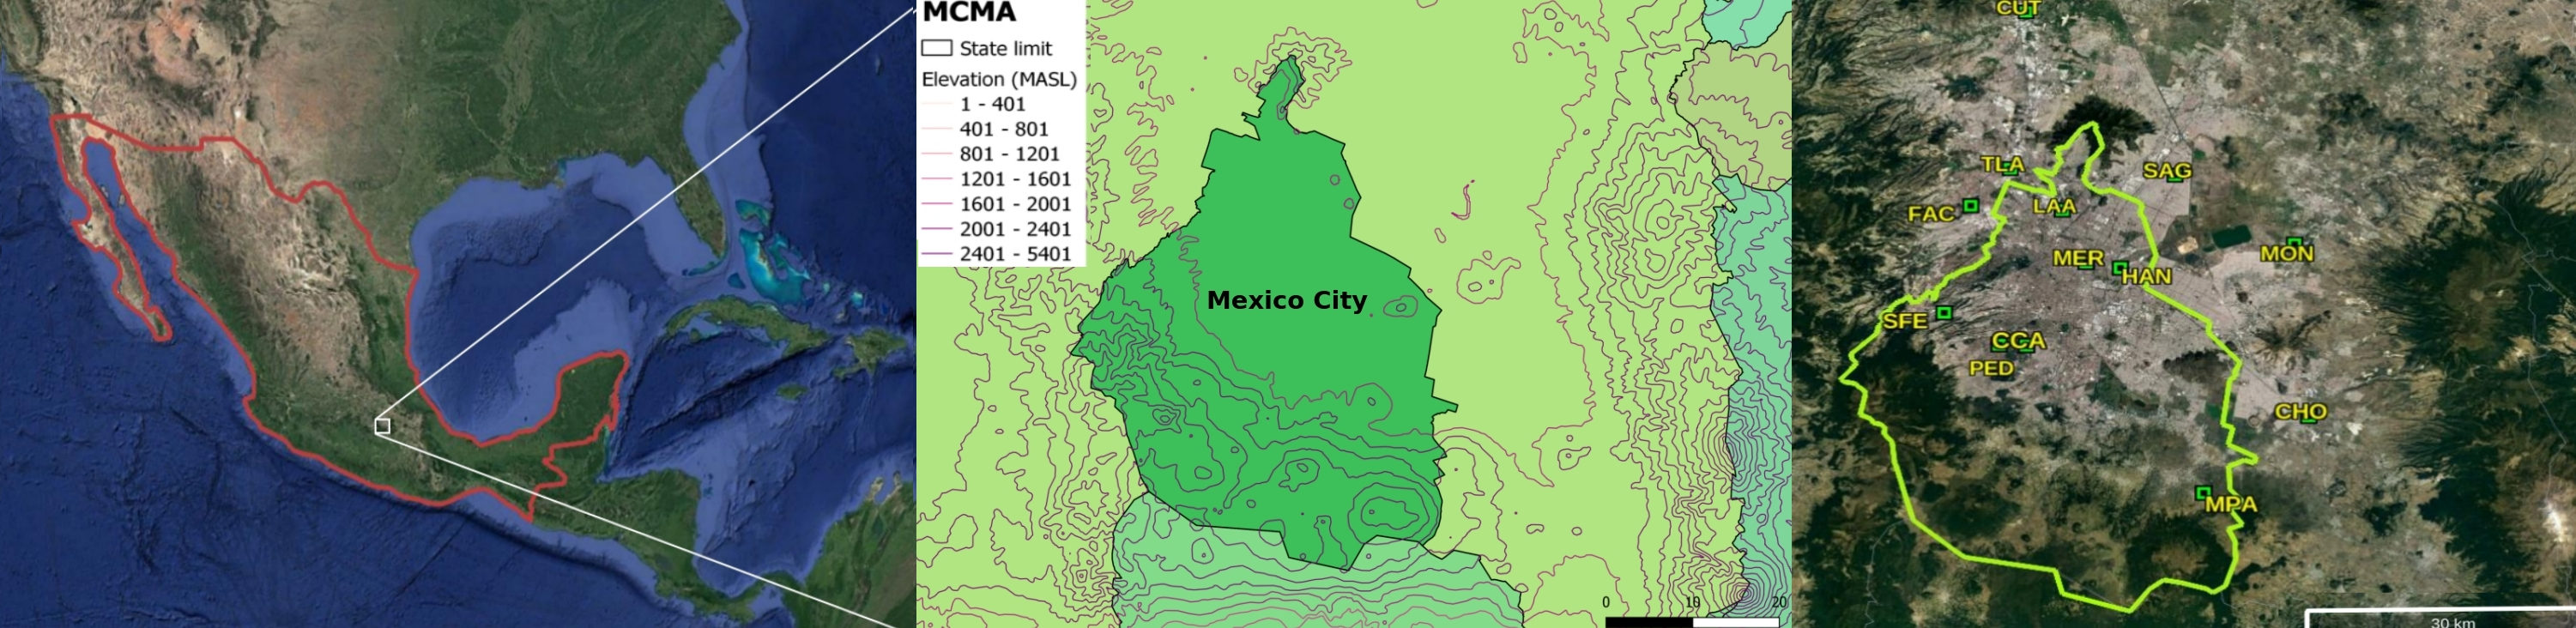
\includegraphics[width=0.84\columnwidth]{cdmx}
\caption{{Maps from left to right: United Mexican States (red contour), Contour
lines scale of Elevation over Mexican Valley (green area) and
Distribution of the stations of the Atmospheric Monitoring System of
Mexico City Government (green contour). Source: Figures at left and
right, Google Earth. Figure at middle, base on CONABIO data
(\href{http://www.conabio.gob.mx/informacion/gis/}{www.conabio.gob.mx/informacion/gis/})
and QGIS.
{\label{547698}}%
}}
\end{center}
\end{figure}

Mexico City has a temperate climate with an extended wet season,
although the rainfall is~relatively high between June and August. The
MCMA is in the~North American Central Time Zone (CT) and uses the
Central Standard Time (CST) i.e. six hours behind Coordinated Universal
Time (UTC). In early spring, the local time changes five hours behind
UTC due to the daylight saving time.

Since the year 2000, UV radiometers installed at the SIMAT network
stations have been measuring erythemally-weighted solar radiation. These
instruments are Model 501-A manufactured by Solar Light Company (SCL)
with sensors detecting wavelengths between 280-400nm. The calibrations
were carried out every year, using a reference sensor by the same
manufacture. Although at the beginning only a few stations were in
operation and have been changing, currently 11 stations are recording
solar erythemal irradiances, which are converted to UV Indices, as given
in Equation 1. The station names are: Chalco (CHA),~Cuautitl\selectlanguage{ngerman}án (CUT),
FES Acatlán (FAC), Hangares (HAN), Laboratorio de Análisis Ambiental
(LAA), Merced (MER), Montecillo (MON), Milpa Alta (MPA), Pedregal (PED),
San Agustín (SAG), Santa Fe (SFE), Centro de Ciencias de la Atmósfera
(CCA) and~Tlalnepantla (TLA). The radiometers of the SIMAT have been
distributed over MCMA, prioritizing the sites with more density of
population, as it is shown in Figure~{\ref{547698}}
right. The coordinates of the stations conforming the~radiometers
network are described in Table 2. On the SIMAT
website~\url{http://www.aire.cdmx.gob.mx/default.php},~UV Index
measurements for each station are available almost in real time.~

Even if there is no SLC radiometer at the station of the Centro de
Ciencias de la Atmósfera (CCA) that belongs to the SIMAT, it has a
photometer of the AErosol RObotic NETwork (AERONET
see~\hyperref[csl:63]{(Holben et al., 1998)}). This instrument measures in situ the Aerosol
Optical Depth (AOD) at 340nm. Additionally, we include measurements from
the Automated Atmospheric Monitoring Network (Red Automática
de~Monitoreo Atmosférico, RAMA), a SIMAT subdivision, that is in charge
of assessing the air quality. These dataset were used to perform a brief
analysis about the criteria pollutants recorded by RAMA: Ozone
(O\textsubscript{3}), carbon monoxide (CO), nitrogen dioxide
(NO\textsubscript{2}) and concentration of particles with diameter less
or equal than 10 \selectlanguage{greek}μ\selectlanguage{english}m (PM\textsubscript{10}). The O\textsubscript{3}~and
NO\textsubscript{2} are reported~in parts per billion (ppb), using
ultraviolet photometry (Teledyne API model 400E) and chemiluminescence
(Teledyne-API model 200E) respectively. The CO in parts per million
(ppm) is derived by absorption of infrared light in a correlation cell
(Teledyne API model 300E) and PM\textsubscript{10}~(in microgram per
cubic meter) is measured by the beta attenuation method (Thermo Model
1405-DF FDMS).\selectlanguage{english}
\begin{table}[H]
\centering
\begin{tabular}{ccccc}
\hline
Station&Environment &Lat (\selectlanguage{ngerman}°N)&Lon (\selectlanguage{ngerman}°W)&El (masl)\\ \hline
CHO &school zone&19.27&99.89&2253\\ 
CUT &ecological park&19.72&99.20&2263\\
FAC &urban&19.48&99.24&2299\\
HAN &urban&19.42&99.08&2235\\
LAA &urban&19.48&99.15&2255\\
MER&downtown&19.42&99.12&2245\\
MON&rural&19.46&98.90&2252\\
MPA&rural&19.18&98.99&2594\\
PED&residential &19.33&99.20&2326\\
SAG&urban&19.53&99.03&2241\\
SFE&residential &19.36&99.26&2599\\
TLA&urban &19.53&99.20&2311\\ 
CCA &University city&  19.33 & 99.18 & 2294\\\hline
\end{tabular}
\caption{{Abbreviations names, environmental descriptor and geographical position of the SIMAT stations placed in MCMA.}}
\end{table}

The available data set is rather larger, spanning two full decades for 5
stations and many years for the others, and with a measurement frequency
of about 1 minute, thus resulting in ca. 2 million data points.
Accordingly, significant averaging was carried out to highlight the main
features of the data.

\subsection*{Satellite data}

{\label{677253}}

Satellite measurements of the Radiative Cloud Factor, the Total Ozone
Column (TOC) and UV Index were used for the current study. These data
were provided by the Ozone Monitoring Instrument (OMI)~on board of
AURA-NASA satellite and the Total~Ozone~Mapping Spectrometer (TOMS) on
board the Earth Probe (EP)-NASA satellite. OMI was created in a
cooperation between the Netherlands Agency for Aerospace Programmes
(NIVR), the Finnish Meteorological Institute (FMI) and NASA. OMI
(hereafter OMI-Aura/NIVR-FMI-NASA) performs observations over a
geographical dimension of 13 \selectlanguage{ngerman}× 24km\textsuperscript{2} at nadir. For
Mexico City, the satellite overpass time is between 19:00h - 21:00h UTC
and data are specific for the coordinates and elevation of Mexico City.
The TOMS-EP/NASA satellite instrument was also considered to complete
the examined period. It is a version that precedes OMI and it was
retrieving~ the TOC from spectral UV measurements. ~

\section*{Measurements analysis}

{\label{833220}}

\emph{Criteria pollutants}{: Ground-based measurements of
PM}\textsubscript{10}{, CO, O}\textsubscript{3}{ and
NO}\textsubscript{2}{ from 11h to 14h CST~were~} extracted from the
SIMAT data{~to compute the daily averages at solar noon and the absolute
maximums.}

\emph{Aerosol Optical Depth:} The~AERONET Aerosol Optical Depth at 340
nm (AOD\textsubscript{340}) data Product Level 2.0 were selected. The
annual averages AOD\textsubscript{340} were calculated from the
continuous measurements during at least 7 months\textsubscript{.}

\emph{Cloud Factor and Total Ozone Column}: The Radiative Cloud Factor
and TOC derived from OMI-Aura/NIVR-FMI-NASA, for the OMTO3 v8.5 dataset,
Collection 3 and L2 quality were collected. The Cloud Factor is
dimensionless, from 0 to 1 for the cloudless days and overcast sky,
respectively. TOC data were obtained from TOMS-EP/NASA. The 1461
observations were acquired of the: TOMS-EP/NASA instrument during the
period 2000 to 2003 and OMI-Aura/NIVR-FMI-NASA data from 2004 to 2019,
both dataset covering the complete time series of the ground-UV Index
measurements.

\emph{UV Index:~}We developed a general code in~\texttt{Python} to
process the hourly averaged UV Index, 24 hours per day, 365 days a year,
along two decades. Hereinafter, we refer to hourly averages simply as UV
Index unless otherwise specified. The script also identifies the maximum
UV index and ignores empty spaces and invalid values, product of the
maintenance of the equipment. The algorithm creates a matrix with the
maximum UV Index (\(UVI_{\max}\)) values sorted by date, hour and
years. It selects the highest UV Index values of the network and a
counter as an extension of the code was executed to quantify the values
and their percentage frequency during 2000-2019 period. Thereupon it
also calculates the hourly, monthly and annual averages. In particular,
the values from 11h to 14h CST~were isolated to compute the daily
averages around solar noon and the absolute maximums. For the UV Index
calculated from OMI-Aura/NIVR-FMI-NASA, we take into account all
available daily values in the period 2000-2019 under the same
specification of the Cloud Factor and TOC data.

\section*{Results and Discussion}

{\label{249401}}

The daily~\(UVI_{\max}\) were selected in the time interval 11:00
h-14:00 h CST from all ground-based measurements over MCMA. The results
indicated that, from a total of 7305 days of continuous
measurements,~the daily~~\(UVI_{max}\) reached values between 6 and
9 on 62.37\% of the days (Figure~{\ref{929259}}). The
highest UV Index values were in the 13-14 range, with a frequency of
less than 1\%.\selectlanguage{english}
\begin{figure}[H]
\begin{center}
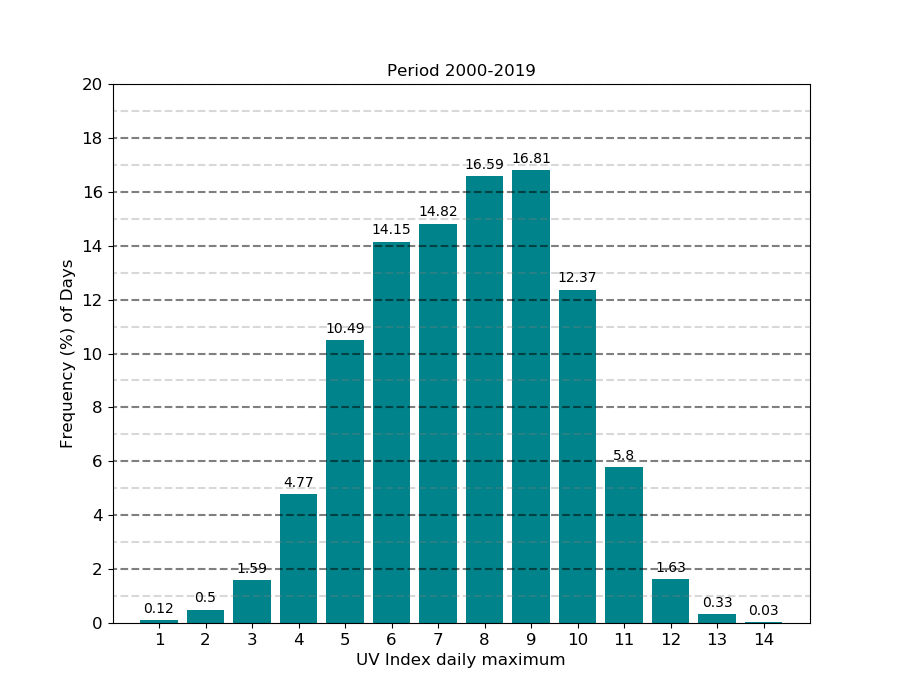
\includegraphics[width=0.56\columnwidth]{HistTotal}
\caption{{Frequency distribution of maximum daily UV Index values in Mexico city
during 2000 -2019.~
{\label{929259}}%
}}
\end{center}
\end{figure}

Figure~{\ref{358425}} shows the diurnal variation of
the UVI for several specific cloud-free days, for different seasons and
several locations. Although the stations are all within a 25 km radius,
substantial differences among them are notable. The differences are
particularly evident in the afternoons, suggesting that their origin is
not related to calibration differences between the instruments.
Photographs of the locations also indicate that shadowing from nearby
structures is not an issue. It is more likely that local differences in
air pollution, particularly aerosols, are the cause of this variability.
Previous studies (e.g.,~\hyperref[csl:14]{(Castro et al., 2001}; \hyperref[csl:13]{Palancar et al., 2013)}) have shown that surface UV
radiation in Mexico City is attenuated significantly by aerosols. The
measurements shown in Figure~{\ref{358425}} are
consistent with increasing pollution during the course of the day, with
highest aerosol loading (and highest variability) attained in the
afternoon. Further support for the role of pollution in suppressing the
UVI comes from the observation made at Santa Fe (SFE) which in
Fig.~{\ref{358425}} are seen to be systematically
higher, e.g. by over 10\% in autumn afternoons, compared to the other
stations. The SFE station is located at 2600 m asl, approximately 300 m
higher than Mexico City downtown, and so avoids a substantial fraction
of the polluted MCMA boundary layer. It is expected to have higher
values of the UVI, in agreement with the observations.\selectlanguage{english}
\begin{figure}[H]
\begin{center}
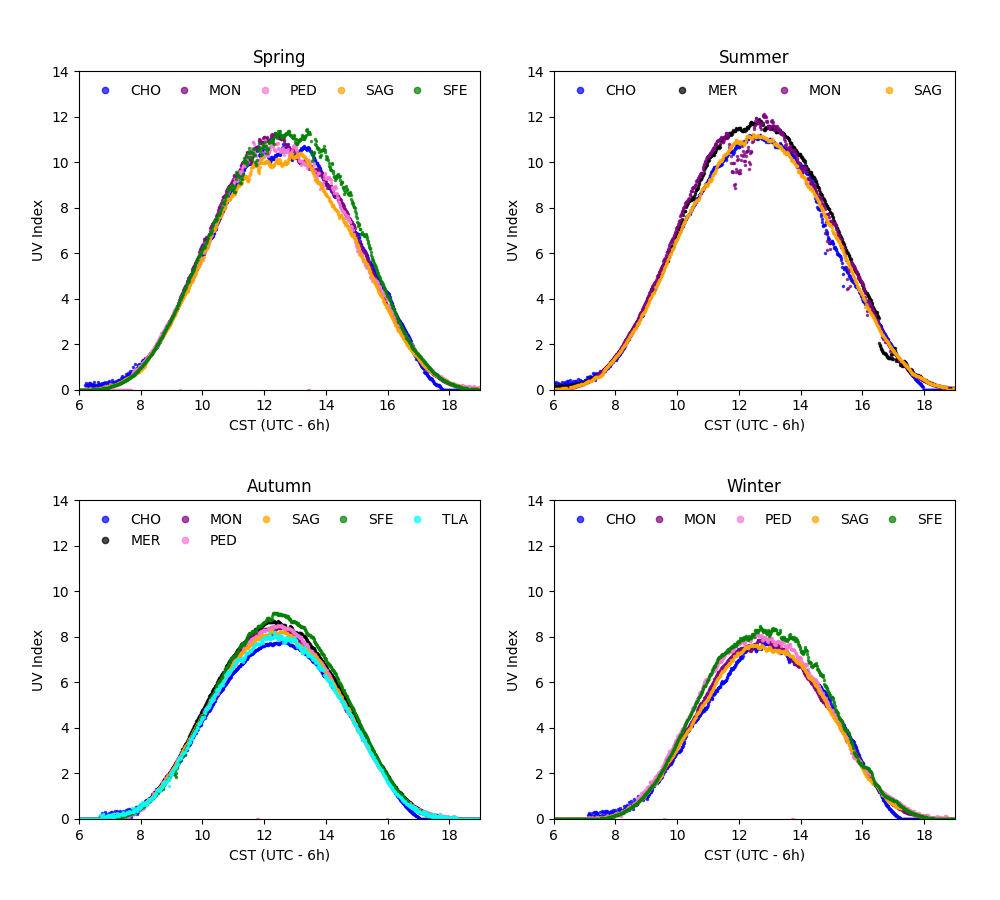
\includegraphics[width=0.98\columnwidth]{season}
\caption{{UV Index measured over MCMA by SIMAT stations each minute along the day
under cloudless conditions~for the seasons and dates (month/day/year):
Spring (04/20/2018), Summer (06/04/2018),~ Autumn (11/13/2018) and
Winter (02/02/2018).
{\label{358425}}%
}}
\end{center}
\end{figure}

Based on ground measurements analysis under all sky conditions we make
an assessment of the values reached around solar noon.~From
daily~\(UVI_{\max}\), the monthly averages (\(\overline{UVI_m}\)) and
Standard Deviations (SD) were
calculated.~The~\texttt{Simple\ Moving\ Average} function
from~\texttt{Python} was applied by quarter and a linear fit along the
two decades was determined (Figure~{\ref{443547}}a).
The linear equation has a slope~\(m_{UVI}\)~of 0.06 per year and
the y-intercept (year 2000) has a UVI value of 8.5. For the sake of
representing an annual behavior, the average, the median, SD, maximum
and minimum of the UV Index were obtained
(Figure~{\ref{443547}}b). The maximum and minimum
monthly mean of the UV Index were 10.6 (in May) and 6.5 (in November),
respectively.\selectlanguage{english}
\begin{figure}[H]
\begin{center}
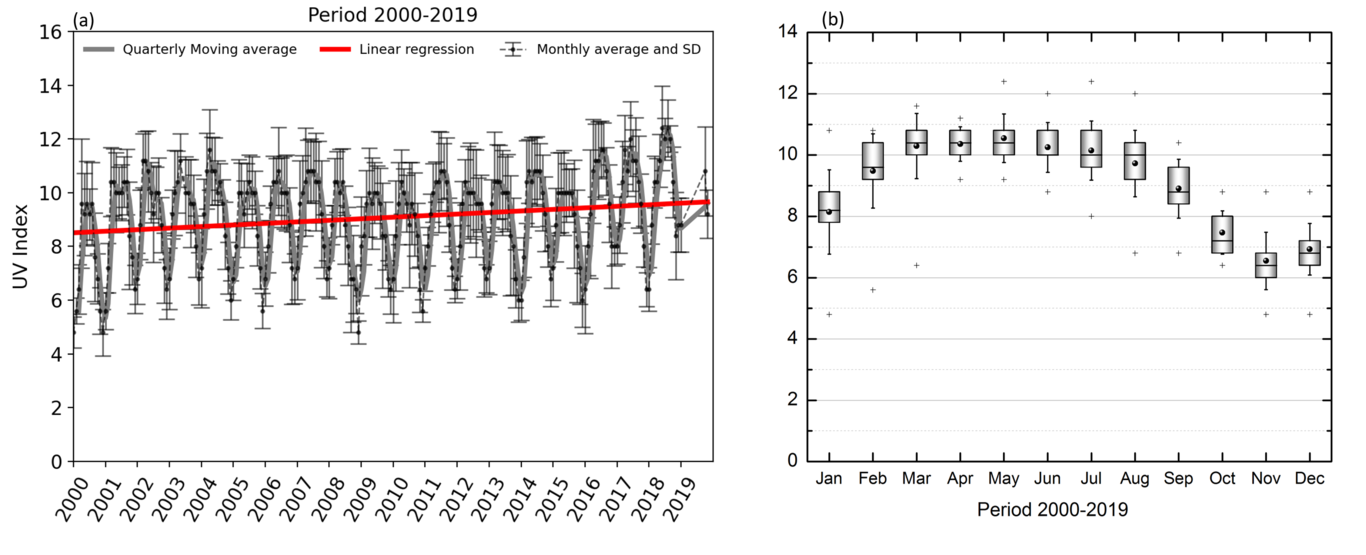
\includegraphics[width=1.00\columnwidth]{AnnualBox}
\caption{{(a) Moving average function (gray curve) quarterly applied to monthly UV
Index and SD (black dots and dash line) and its linear fit (red line).
(b) Boxplot of monthly UV Index in the period 2000-2019: median (central
bold line), average (black dot), 25\textsuperscript{th} and
75\textsuperscript{th}~percentiles (box edges), Standard Deviation (the
whiskers) and the minimum and maximum values(plus sign).
{\label{443547}}%
}}
\end{center}
\end{figure}

In January the median and mean UVI values are near 8 (see
Fig.~{\ref{443547}}b). However, the UVI values and SD
seems to be flattened (in the range 10-11) from March to August and
decreasing to November (rainy period) with a slight rise on December.
The rather low monthly UV Index values, may be a consequence of
averaging measurements in presence of clouds and/or significant
pollution. Both depend on time of the year, with a cool dry season from
November to February, warm dry March-April-May, and a rainy season
from~June to October. In addition to urban aerosol pollution sources,
biomass burning for agriculture and wood cooking also contribute to poor
air quality in the MCMA~\hyperref[csl:64]{(Retama et al., 2015)}. In the warm season, faster
photochemical oxidant formation, dust, and biomass burning all
contribute to strong aerosol loading. In rainy months, UV Index values
are lower due to the presence of clouds.~

For assessing the influence of the aerosols and criteria pollutants in
the UV Index, we processed the PM\textsubscript{10}, CO,
NO\textsubscript{2}, O\textsubscript{3}~and AOD\textsubscript{340}
ground-based measurements carried out at the stations mentioned in Table
2. From daily measurements from 11h to 14h CST the annual mean of
PM\textsubscript{10}, CO, NO\textsubscript{2}, O\textsubscript{3} were
calculated. For the case of the AOD\textsubscript{340}, the measurements
along of the day were averaged. Figure~{\ref{610674}}{
shows the trends of the annual values from 2000 to 2019. On the other
hand, to estimate the percentage~change per year (}\(\epsilon\left(\%\right)\)),
the slope (\(m_ {X}\)) of~ the linear fit and the average~in all
period (\(\overline{X}_{2000-2019}\)) were used. In the case of the UVI
percentage~change was 0.66 \% per year. In the same way, Table 3 shows
the values corresponding to PM\textsubscript{10}, CO,
NO\textsubscript{2}, O\textsubscript{3} and AOD\textsubscript{340}.~\selectlanguage{english}
\begin{figure}[H]
\begin{center}
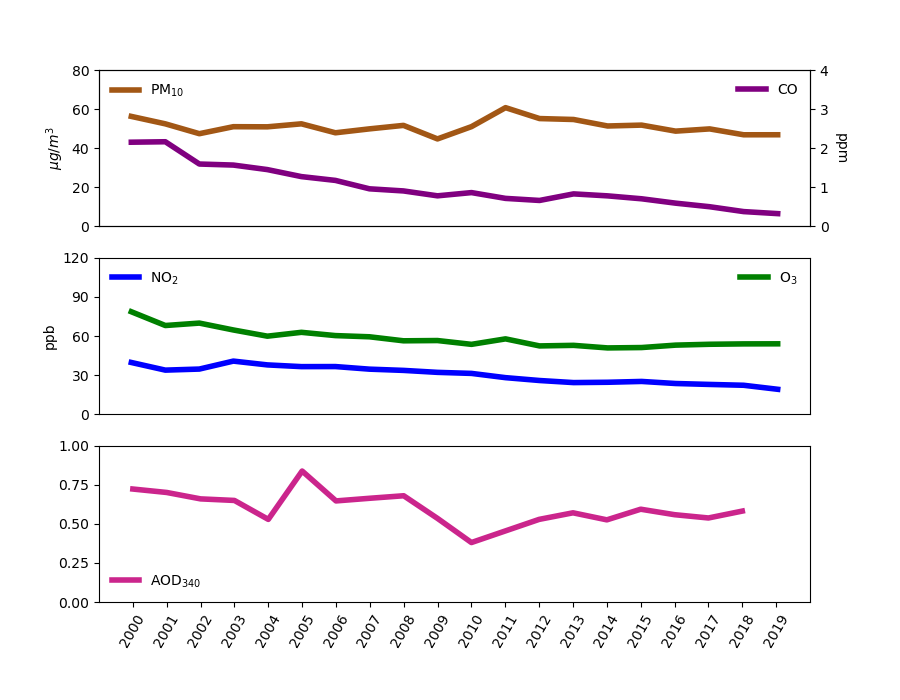
\includegraphics[width=0.56\columnwidth]{contCDMX}
\caption{{Air quality trends for the period 2000-2019 in Mexico City Metropolitan
Area from annual averages obtained between 11h to 14h CST every
day:~PM\textsubscript{10~}(brown curve),~ CO (purple curve),
NO\textsubscript{2~}(blue curve), O\textsubscript{3}~(green curve) and
AOD\textsubscript{340~}(pink curve).
{\label{610674}}%
}}
\end{center}
\end{figure}

Policies aimed on the improvement of air quality simultaneously with
urban and industrial development have taken place in the last
years~\hyperref[csl:65]{(Molina et al., 2009)}. Stephens et al (2008) determined the monthly
variation of the concentrations of PM\textsubscript{10} in the morning
(between 7-12h CTS) and O\textsubscript{3} in the afternoon (from 11h to
17h CTS) for the years 2001--2007 with a negative
trend~\hyperref[csl:66]{(Stephens et al., 2008)}. These results revel that the decreasing of
criteria pollutants could be the cause of the slight increase in the UV
index trend. Nevertheless, MCMA has a large period under typical
cloudiness days or wet season, in general from June to November.\selectlanguage{english}
\begin{table}[H]
\centering
\begin{tabular}{cccc} \hline
Name &$m_X$ & $\overline{X}_{2000-2019}$ & $\epsilon(\%)$\\ \hline
UVI &0.06 &9.085 &0.66 \\
PM$_{10}$ &-0.1196 & 51.11& -0.23\\ 
CO &-0.0835 &1.02 &-8.18\\ 
NO$_2$ &-1.04 & 30.35 &-3.43\\ 
O$_3$ &-1.046 & 58.48 &-1.79\\ 
AOD$_{340}$ &-0.01 &0.60 &-1.67\\
\hline
\end{tabular}
\caption{{UV Index and criteria pollutants: slope from linear fit, average 2000-2019 in units of $\mu g/m^3$(PM$_{10}$), ppm (CO), ppb (NO$_2$ and O$_3$) and dimensionless (UV Index and AOD$_{340}$) and annual percentage change (\%/year)}}
\end{table}

A fundamental issue is to establish the clouds influence on the mean UV
Index values. C{loudy days are frequent almost all year in MCMA. The
attenuation on~\(UVI_{\max}\)~by clouds could also be predominant
out of the rainy period.~However,~a gap in our knowledge is to
discriminate cloudy days only using hourly UV Index measured in situ.
T}he Radiative Cloud Factor measurements by OMI-Aura/NIVR-FMI-NASA
satellite instrument was extracted for the Mexico City coordinates.
Figure~{\ref{573921}}a depicts the daily Cloud Factor
(5844 observations) recorded from 2004 to 2019 period. It revealed that
cloud cover regularly appears in part of the warm dry and rainy seasons,
and is frequent the rest of the months.~

Moreover, to incorporate satellite information about the total ozone
column (TOC) is fundamental for understanding the UV Index levels.
Regarding the cold dry period (December to February) TOMS-EP/NASA and
OMI-Aura/NIVR-FMI-NASA instruments estimated the lowest clouds coverage
as well as the lowest TOC (Figure {\ref{573921}}b).
Conversely, higher ozone levels were registered from April to
September.~\selectlanguage{english}
\begin{figure}[H]
\begin{center}
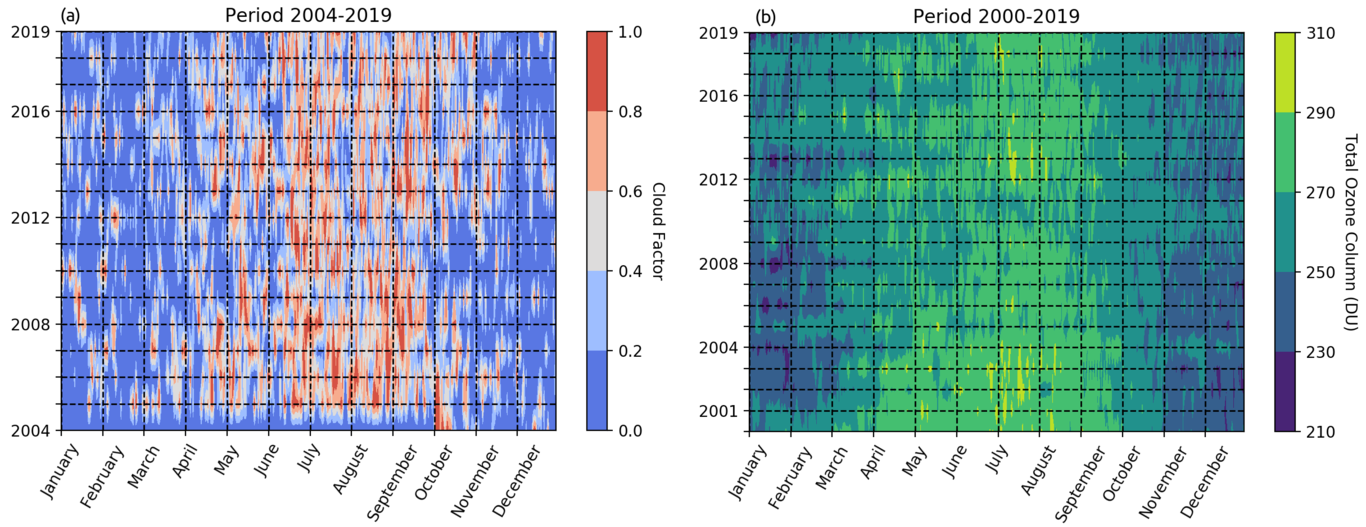
\includegraphics[width=1.00\columnwidth]{OzonoCloudDaily}
\caption{{Satellite data over Mexico City: (a) Cloud Factor OMI-Aura/NIVR-FMI-NASA
between 2004-2019 and (b) Total Ozone Column from TOMS-EP/NASA and
OMI-Aura/NIVR-FMI-NASA in the periods 2000-2003 and 2004-2019,
respectively.
{\label{573921}}%
}}
\end{center}
\end{figure}

To compare the ground-base measurements at solar noon, the UV Index
measured by OMI-Aura/NIVR-FMI-NASA were mapped.
Figure~{\ref{674611}}~represents the satellite UV Index
data from 2005 to 2019 (there was no previous data in the analyzed
period). As can be seen, the levels are higher than the monthly averages
shown in Figure~{\ref{443547}}~(where the UVI maximum
values barely exceed 11). From the~middle~of January to mid-November,
the satellite UV Index varies from 8 up to about 15
(\(UVI_{\max}=14.9\)). In particular, values equal or larger than 11,
corresponding to the \emph{Extreme} qualification for the UV index given
by WHO, are commons from April to September.\selectlanguage{english}
\begin{figure}[H]
\begin{center}
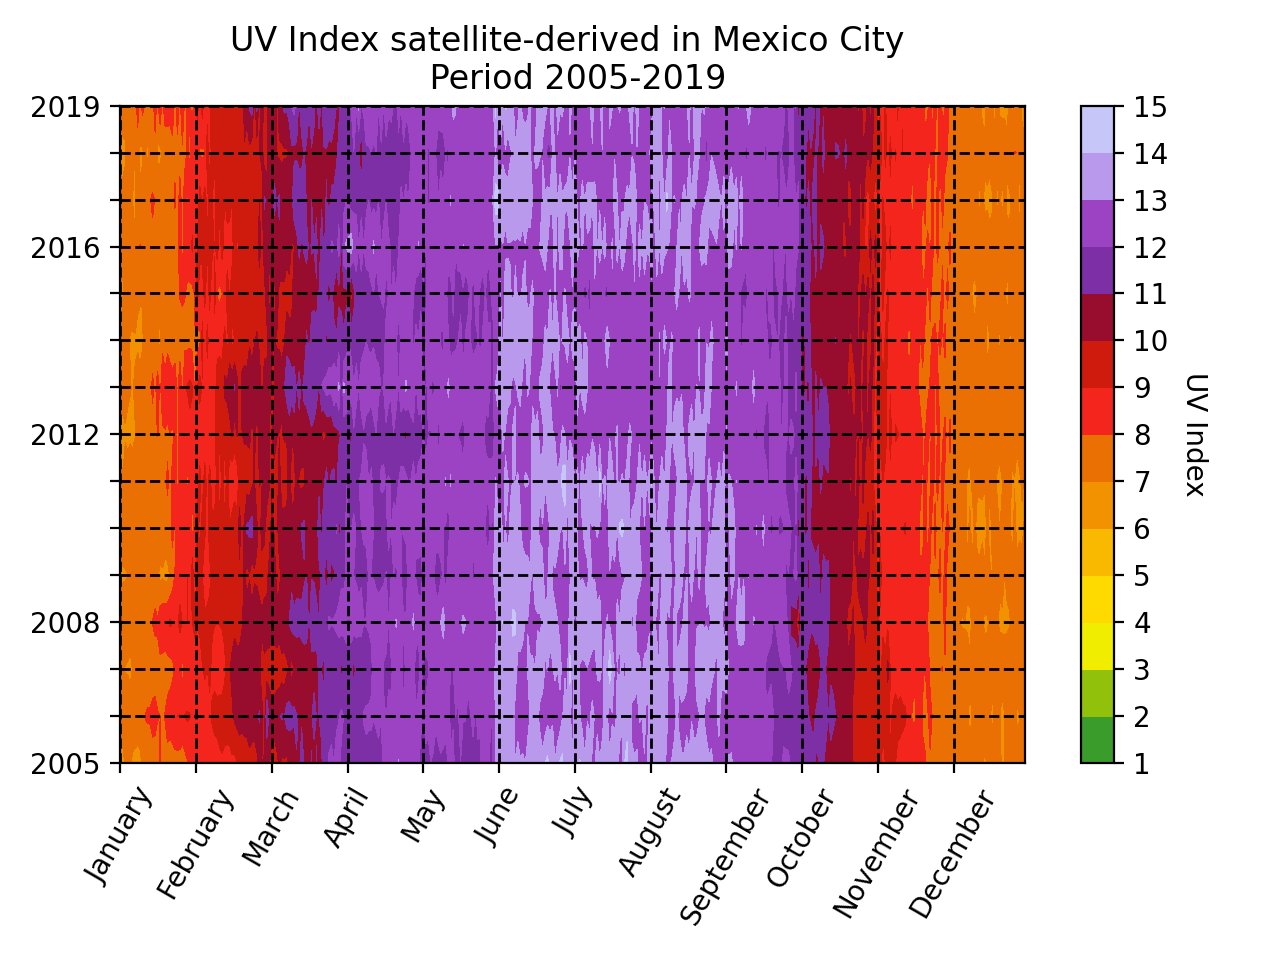
\includegraphics[width=0.70\columnwidth]{UVI-OMI}
\caption{{UV Index recorded by~OMI-Aura/NIVR-FMI-NASA, from 2005 to 2019.
{\label{674611}}%
}}
\end{center}
\end{figure}

The UVI derived from satellite observations is seen to be systematically
larger than the mean UVI values measured at the ground. This is to some
extent expected, since satellites fail to resolve local clouds and
aerosols, particularly near surface levels. To examine this
over-estimation in more detail, we selected a subset of the ground-based
data that included only the maximum value from all stations and all
years of measurement, for each hour and day of the year. The result for
the compilation of this~~\(UVI_{\max}\)~is illustrated in
Figure~{\ref{931769}}.~It can be seen
that~\(UVI_{\max}\ge8\ \) is very frequent at solar noon, as was seen in
Figure~{\ref{929259}}, corresponding to the daily
maximum near noon. The highest~\(UVI_{\max}\) recorded in the period
2000-2019 was 14.9, which is consistent with the maximum values obtained
from satellite observations.\selectlanguage{english}
\begin{figure}[H]
\begin{center}
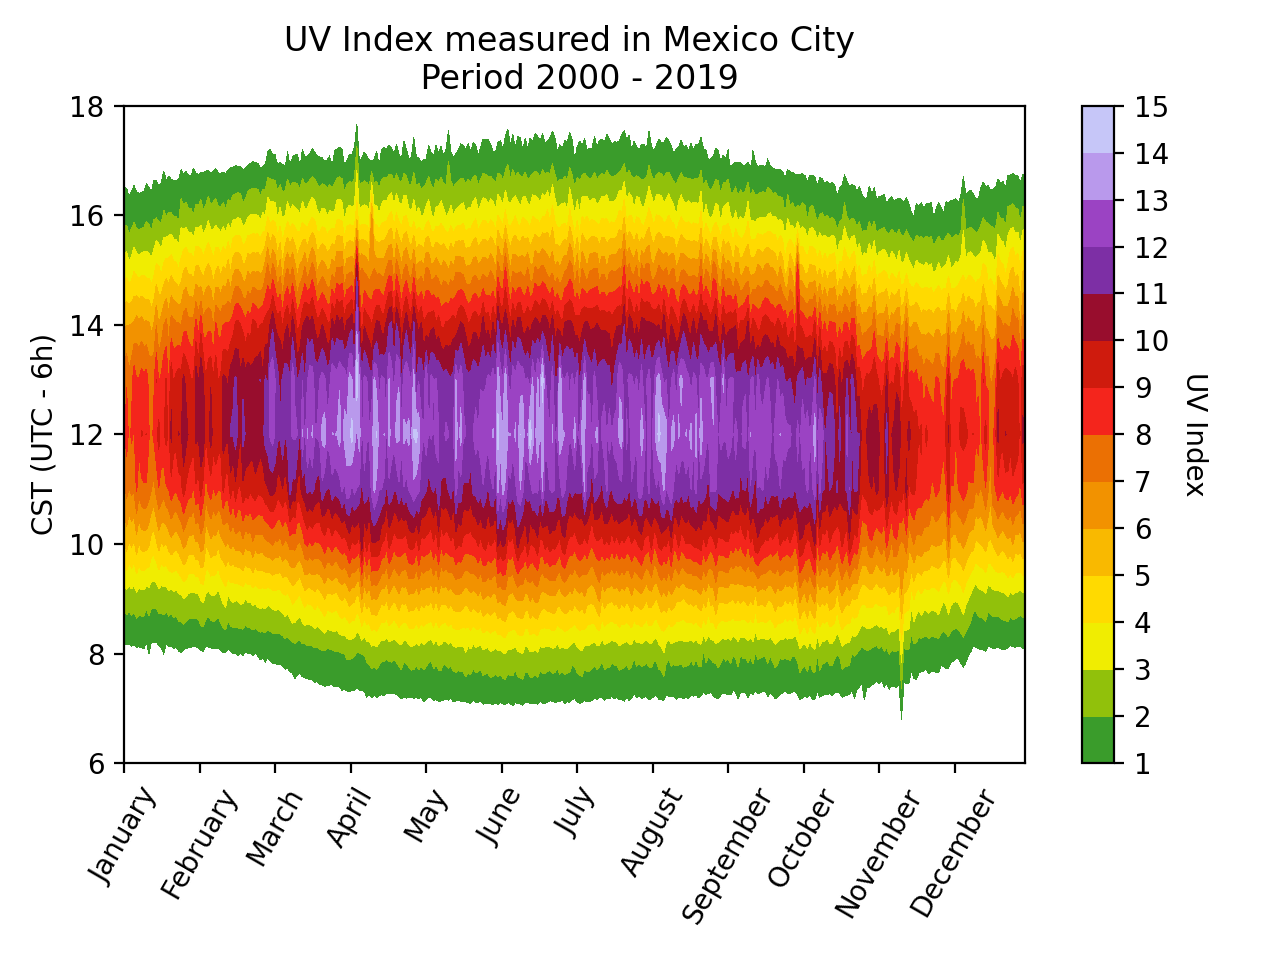
\includegraphics[width=0.98\columnwidth]{MaxUVindex}
\caption{{The highest UV Index values recorded during 2000-2019, for each day of
the year and each hour of the day. Selected from SIMAT observations in
Mexico City.~
{\label{931769}}%
}}
\end{center}
\end{figure}

However, this comparison also suggests that satellite data estimate may
be biased to low values under some conditions. The most noticeable
difference is in December, when the~\(UVI_{\max}\) in situ are
between 8-11 and satellite data ranging from 6 to 8.~

A visual screening process was applied to the ground measurements to
separate cloudless and cloudy conditions, as automated methods are still
challenging~\hyperref[csl:67]{(Badosa et al., 2014}; \hyperref[csl:68]{Wild et al., 2019)}. In spite of the lack of information
about the presence of clouds during the day, the data acquired each
minute in the period 2016-2018 were a great identification tool. The
measurements behavior minute by minute was used to recognize clear sky
days. As expected, the monthly averages UV Index under cloudless sky
were higher than~\(\overline{UVI}_m\), probably due to the clouds absence.\selectlanguage{english}
\begin{figure}[H]
\begin{center}
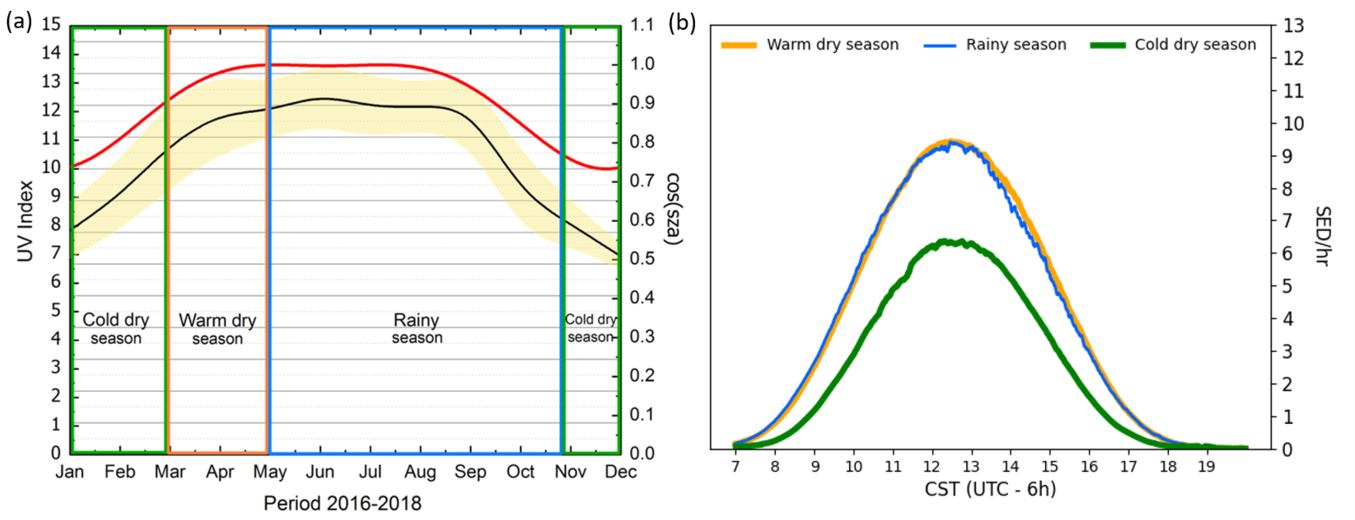
\includegraphics[width=0.98\columnwidth]{season_graphics}
\caption{{Seasonal variability of the UV Index from ground measurement under
cloudless sky in cold dry season (green), warm dry season (orange) and
rainy season (blue) for: (a) Interpolation of the monthly mean UV Index
(and respective SD in wide yellow bands) at solar noon in the period
2016-2018 (black curve),~and cos(sza) at solar noon (red curve)~and (b)
Daily averages of the SED/hr~along the hours of the day, for each
season.~
{\label{590688}}%
}}
\end{center}
\end{figure}

The SIMAT publishes a recommendation of protection according to the
measured UVI. In this way, it would be more convenient to estimate in
term of SED/hr and then, to derive the exposure times.
The~\(H_{er}\) expressed as function of time can be obtained~
(by combing Eqs. 1 and 2)

\begin{equation}
  \frac{SED}{hr}=0.9UVI.  
\end{equation}
As is indicated in
Figure~{\ref{590688}}a, the interpolation of the UV
Index (and corresponding SED/hr) at solar noon under clear sky, revels
that these levels match better with the~\(UVI_{\max}\) values
measured over the network (see Figure~{\ref{931769}})
and the highest UV Index value of 12.6 (11.3 SED/hr) in June.
Additionally, the SED/hr under all clear sky days were averaged for the
three seasons: cold dry, warm dry and rainy, as is shown in
Figure~{\ref{590688}}b. The warm dry and rainy seasons
have a behavior almost coincident. Few data under clear sky were
detected between September and October (part of the rainy season) being
a negligible contribution on total average just when the UV Index
decrease. Nevertheless, the daily asymmetries around solar noon shown in
Figure~{\ref{358425}} could be caused by criteria gases
and aerosol. An additional comparison between AOD ground-based
measurements and derived data from model~\hyperref[csl:14]{(Castro et al., 2001}; \hyperref[csl:69]{Cabrera et al., 2012}; \hyperref[csl:13]{Palancar et al., 2013)}~are needed
to confirm this hypothesis.~ However, the main reason for the seasonal
variation of the cloud-free UVI is not due to aerosols, but rather
simply to the annual cycle of the solar zenith angle, the cosine of
which is also plotted in Fig.~{\ref{590688}}a and is
seen to correlate well with the UVI. ~

As was mentioned in the Introduction, the phototypes III and IV are the
most frequents in Mexican inhabitants. The code in~\texttt{Python}~was
executed to compute the accumulate doses~\(H_{er}\)~by means of
Equation 2. Particularly, the solar exposure time as function of the
local hour (considering only clear sky days in the period 2016-2018)
were estimated for~the skin types III and IV by means the repetitive
operation until reach 3.0 SED and 4.5 SED, respectively.
Figure~{\ref{276646}}~illustrates the result of
exposure time to accumulate the~corresponding~\(H_{er}\)~for
each phototype.\selectlanguage{english}
\begin{figure}[H]
\begin{center}
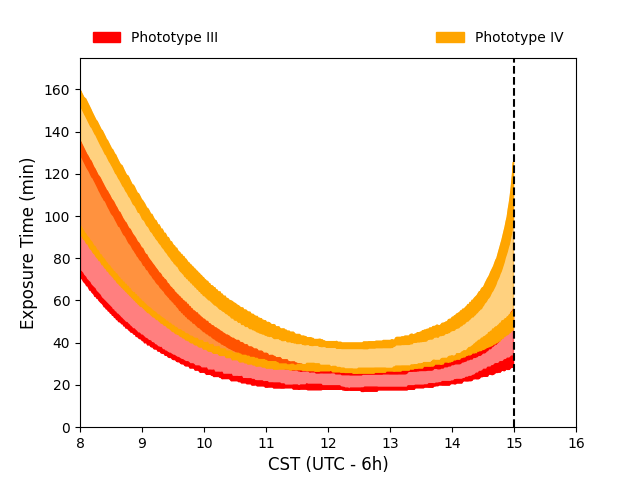
\includegraphics[width=0.70\columnwidth]{FillDosis2}
\caption{{Solar Exposure Time along of the hours of the day for typical skin type
of the Mexican population to accumulate~\(H_{er}\): 3.0 SED for
phototype III (red curves) and and 4.5 SED for phototype IV (yellow
curves). Enveloping curves represent the limit times in summer (lower
curve) and winter (higher curve). Dotted lines at 15h CST detail the
final time when the minimal erythemal dose cannot be reached.
{\label{276646}}%
}}
\end{center}
\end{figure}

The upper and lower wide curves are associated to measurements carried
out in summer and winter seasons and the areas contain the exposure
times between spring and autumn. The asymptote at 15h CTS represents
that it will not be possible to achieve the MED after this hour. The
representation along the hours shows that the exposure time range was
narrower, since in this case only clear sky measurements we considered.

\section*{Conclusion}

{\label{507127}}

The aim of this study was characterize the UV Index reached over Mexico
City Metropolitan Area in the last 20 years. The location of this
megacity is in a region prone to achieve high values of UV
Index~\hyperref[csl:27]{(Tanskanen \textit{et al.}, 2006}; \hyperref[csl:26]{Zaratti \textit{et al.}, 2014)}. In spite of Mexico City high altitude (2240 m
asl) the ultraviolet irradiance is lower than in Colima (485 m asl), a
relatively pollution-free city and placed at~about the same
latitude~\hyperref[csl:19]{(Galindo \textit{et al.}, 1995)}. The~\(\overline{UVI}_m\)~at solar noon
reaches up to 10.6 obtained under all sky conditions (see
Figure~{\ref{443547}}). In contrast, UV Index from
satellite data (Figure~{\ref{674611}}) and the
highest~\(UVI_{\max}\) ground-based values were 14.9 (in
Figure~{\ref{931769}}), both in \emph{Extreme}
qualification range of WHO~\hyperref[csl:24]{(WHO, 2002)}. The high aerosols
concentration and smog photochemistry products may affect the solar
radiation reaching the surface~\hyperref[csl:14]{(Castro \textit{et al.}, 2001}; \hyperref[csl:13]{Palancar \textit{et al.}, 2013)}. Also the existence of
cloud coverage almost all year round can be partially responsible for
the not as high as expected UV index values for Mexico city. In the
period 2000-2019 the criteria pollutants trends:~PM\textsubscript{10},
CO, NO\textsubscript{2}, O\textsubscript{3} and
AOD\textsubscript{340~}~were negatives. However
the~\(\overline{UVI}_m\)~at solar noon under all sky conditions are in
the\emph{~High, Very High and Extreme}~ranges (\(\overline{UVI}\ \ge6\))
during all months of the year (see
Figures~{\ref{443547}},~{\ref{674611}}
and~{\ref{931769}}). The few articles existing about
solar radiation in this city have either been short-term studies or have
not focused on UV irradiance affecting health skin. In this work, a code
in~\texttt{Python}~was created to analyze the complete database at
different scales of time (minute, hours, days and years) calculating the
averages and the maximums UV Index as well and its trend. One part of
the script was extended to the management and determination of the
exposure times corresponding~ to the threshold erythemal dose. The
levels of UV Index at noon in the period 2000~to 2019 over MCMA show a
trend of 0.66 \% per year with respect to the mean.~This trend is within
the range of the results published by Herman (2010) about erythemal
irradiance trend from 1979 to 2008 derived from satellite data (between
-1.7\% to 2.0\% annually) in the latitudinal range of Mexico City. The
current study also contributes to the determination of the solar
exposure time as a limit to avoid sunburn, considering the phototypes
more frequent of the inhabitants of the Mexico City. Regarding to skin
color to define the sensibility, imprecise terminology such as `ethnic
skin' and `Hispanic skin' accentuates the problem of sparse data and
hides relevant characteristics. There are discrepancies between the MED
values defined for each phototype~\selectlanguage{ngerman}\hyperref[csl:30]{(Fitzpatrick, 1988}; \hyperref[csl:72]{Sanclemente \textit{et al.}, 2008}; \hyperref[csl:31]{Pérez \textit{et al.}, 2014}; \hyperref[csl:33]{Lehmann \textit{et al.}, 2019}; \hyperref[csl:64]{Cadet \textit{et al.}, 2019)}. The definition of
the colors gradient and the descriptive numbers associated to the
phototypes should always be clear and specific. An essential element is
assuming ethnic diversity. The threshold erythemal dose for each
phototype is fundamental to awareness of the photoprotection. The
photoprotection needs to be promoted with properly communication about
the risk and skin care. This premise would help to demystify the
perception about the fact that the darker skins can not have sunburn or
are exempt to develop skin-cancer~\hyperref[csl:41]{(Castanedo-Cazares \textit{et al.}, 2006)}. Prevention and
timely diagnosis continue to be the main strategy to reduce the
incidence and impact of skin cancer~\hyperref[csl:73]{(Pinedo \textit{et al.}, 2009}; \hyperref[csl:74]{Alfaro-Sánchez \textit{et al.}, 2016)}. This study
highlights the importance of knowing the UV Index levels and the maximum
exposure times to avoid damage. The prevention campaigns may be
accompanied by recommendations associated with typical customs of the
country, such as the use of hats and long-sleeved shirts when they work
or perform recreational activities in outdoors conditions.~This UV Index
assesment can also be of interest for applications in the use of solar
energy, validation of radiative transfer models and satellite
measurements, as well as monitoring of pollutants absorbing in the UV
range.

\section*{Acknowledgements}

{\label{667124}}

We wish to acknowledge the SEDEMA members, institution that belongs to
the Mexico City Government. We would like to express special gratitude
to Q. Armando Retama for his great job in the management data network
and constant advisory. Adriana Ipiña would like to extend her thanks
to\textbf{~}Dirección General de Personal Académico, Universidad
Nacional Autónoma~de México (DGAPA-UNAM) for the postdoctoral fellowship
at Centro de Ciencias~de la Atmósfera of the UNAM.~Rubén D Piacentini
wishes to thank CONICET and National University of Rosario, Argentina,
for their partial support to the present work.~The National Center for
Atmospheric Research is sponsored by the National Science Foundation.



~

\selectlanguage{english}
\FloatBarrier
\section*{References}\sloppy
\phantomsection
\label{csl:18}Acosta LR, Evans WFJ. 2000. {Design of the Mexico City {UV} monitoring network: {UV}-B measurements at ground level in the urban environment}. \textit{Journal of Geophysical Research: Atmospheres}. American Geophysical Union ({AGU}), 105(D4): 5017–5026. \url{https://doi.org/10.1029/1999jd900250.}

\phantomsection
\label{csl:74}Alfaro-Sánchez A, García-Hidalgo L, Casados-Vergara R, Rodríguez-Cabral R, Piña-Osuna AK, Sánchez-Ramos A. 2016. {Cáncer de piel. Epidemiología y variedades histológicas, estudio de cinco años en el noreste de México}. \textit{Dermatol Rev Mex.}, 60(2).

\phantomsection
\label{csl:69}Badosa J, Calbó J, Mckenzie R, Liley B, González JA, Forgan B, Long CN. 2014. {Two methods for retrieving UV index for all cloud conditions from sky imager products or total SW radiation measurements.}. \textit{Photochem Photobiol}, 90: 941–51.

\phantomsection
\label{csl:59}Bech J, Sola Y, Oss{\'{o}} A, Lorente J. 2014. {Analysis of 14 years of broadband ground-based solar {UV} index observations in Barcelona}. \textit{International Journal of Climatology}. Wiley, 35(1): 45–56. \url{https://doi.org/10.1002/joc.3961.}

\phantomsection
\label{csl:43}Bino SD, Bernerd F. 2013. {Variations in skin colour and the biological consequences of ultraviolet radiation exposure}. \textit{British Journal of Dermatology}. Wiley, 169: 33–40. \url{https://doi.org/10.1111/bjd.12529.}

\phantomsection
\label{csl:29}Braslavsky SE. 2007. {Glossary of terms used in photochemistry 3rd edition ({IUPAC} Recommendations 2006)}. \textit{Pure and Applied Chemistry}. Walter de Gruyter {GmbH}, 79(3): 293–465. \url{https://doi.org/10.1351/pac200779030293.}

\phantomsection
\label{csl:23}CIE. 2014. \textit{{Rationalizing Nomenclature for UV dose and effects on humans}}. The International Commission on Illumination and World Meteorological Organization.

\phantomsection
\label{csl:71}Cabrera S, Ipi{\~{n}}a A, Damiani A, Cordero RR, Piacentini RD. 2012. {{UV} index values and trends in Santiago Chile (33.5{\textdegree}S) based on ground and satellite data}. \textit{Journal of Photochemistry and Photobiology B: Biology}. Elsevier {BV}, 115: 73–84. \url{https://doi.org/10.1016/j.jphotobiol.2012.06.013.}

\phantomsection
\label{csl:64}Cadet J-M, Bencherif H, du Preez DJ, Portafaix T, Sultan-Bichat N, Belus M, Brogniez C, Auriol F, Metzger J-M, Ncongwane K, Coetzee GJR, Wright CY. 2019. {Solar {UV} Radiation in Saint-Denis La R{\'{e}}union and Cape Town, South Africa: 10 years Climatology and Human Exposure Assessment at Altitude}. \textit{Atmosphere}. {MDPI} {AG}, 10(10): 589. \url{https://doi.org/10.3390/atmos10100589.}

\phantomsection
\label{csl:41}Castanedo-Cazares JP, Torres-Álvarez B, Medellín-Pérez ME, Aguilar-Hernández GA, Moncada B. 2006. {Conocimientos y actitudes de la población mexicana con respecto a la radiación solar}. \textit{Gaceta Médica de México}, 142.

\phantomsection
\label{csl:40}Castanedo-Cázares JP, Torres-Álvarez B, Ondarza SS, Pérez AE, Moscoso AG. 2012. {Estimación del tiempo de exposición solar para quemadura en población mexicana}. \textit{Gaceta Médica de México}, 148.

\phantomsection
\label{csl:14}Castro T, Madronich S, Rivale S, Muhlia A, Mar B. 2001. {The influence of aerosols on photochemical smog in Mexico City}. \textit{Atmospheric Environment}. Elsevier {BV}, 35(10): 1765–1772. \url{https://doi.org/10.1016/s1352-2310(00)00449-0.}

\phantomsection
\label{csl:25}Cede A, Luccini E, Nuñez L, Piacentini RD, Blumthaler M. 2002. {Monitoring of erythemal irradiance in the Argentine ultraviolet network}. \textit{Journal of Geophysical Research}. American Geophysical Union ({AGU}), 107(D13). \url{https://doi.org/10.1029/2001jd001206.}

\phantomsection
\label{csl:21}Corr CA, Krotkov N, Madronich S, Slusser JR, Holben B, Gao W, Flynn J, Lefer B, Kreidenweis SM. 2009. {Retrieval of aerosol single scattering albedo at ultraviolet wavelengths at the T1 site during {MILAGRO}}. \textit{Atmospheric Chemistry and Physics}. Copernicus {GmbH}, 9(15): 5813–5827. \url{https://doi.org/10.5194/acp-9-5813-2009.}

\phantomsection
\label{csl:47}Cuevas AG, Dawson BA, Williams DR. 2016. {Race and Skin Color in Latino Health: An Analytic Review}. \textit{American Journal of Public Health}. American Public Health Association, 106(12): 2131–2136. \url{https://doi.org/10.2105/ajph.2016.303452.}

\phantomsection
\label{csl:12}Dickerson RR. 1997. {The Impact of Aerosols on Solar Ultraviolet Radiation and Photochemical Smog}. \textit{Science}. American Association for the Advancement of Science ({AAAS}), 278(5339): 827–830. \url{https://doi.org/10.1126/science.278.5339.827.}

\phantomsection
\label{csl:2}Doran JC, Abbott S, Archuleta J, Bian X, Chow J, Coauthors. 1998. {The IMADA-AVER Boundary Layer Experiment in the Mexico City Area}. \textit{Bull. Amer. Meteor. Soc.}, 79.

\phantomsection
\label{csl:50}ENADIS. 2017. \textit{{Encuesta Nacional sobre Discriminación}}. CONAPRED and INEGI.

\phantomsection
\label{csl:11}Finlayson-Pitts BJ, Pitts JN. 2000. \textit{{Chemistry of the Upper and Lower Atmosphere}}. Elsevier, xvii--xviii.

\phantomsection
\label{csl:56}Fioletov VE, Kimlin MG, Krotkov N, McArthur LJB, Kerr JB, Wardle DI, Herman JR, Meltzer R, Mathews TW, Kaurola J. 2004. {{UV} index climatology over the United States and Canada from ground-based and satellite estimates}. \textit{Journal of Geophysical Research: Atmospheres}. American Geophysical Union ({AGU}), 109(D22): n/a--n/a. \url{https://doi.org/10.1029/2004jd004820.}

\phantomsection
\label{csl:22}Fitzpatrick TB. 1974. \textit{{Sunlight and man: An introduction to the problem of normal and abnormal of responses man's skin to solar radiation}}. University of Tokyo Press.

\phantomsection
\label{csl:30}Fitzpatrick TB. 1988. {The validity and practicality of sun-reactive skin types I through VI.}. \textit{Arch Dermatol}, 124: 869–71.

\phantomsection
\label{csl:15}Galindo I, Castro S, Valdes M. 1991. {Satellite derived solar irradiance over Mexico}. \textit{Atmósfera}, 4.

\phantomsection
\label{csl:19}Galindo I, Frenk S, Bravo H. 1995. {Ultraviolet Irradiance over Mexico City}. \textit{Journal of the Air {\&} Waste Management Association}. Informa {UK} Limited, 45(11): 886–892. \url{https://doi.org/10.1080/10473289.1995.10467419.}

\phantomsection
\label{csl:20}Goering CD. 2005. {Simultaneous retrievals of column ozone and aerosol optical properties from direct and diffuse solar irradiance measurements}. \textit{Journal of Geophysical Research}. American Geophysical Union ({AGU}), 110(D5). \url{https://doi.org/10.1029/2004jd005330.}

\phantomsection
\label{csl:28}Herman JR. 2010. {Global increase in {UV} irradiance during the past 30 years (1979{\textendash}2008) estimated from satellite data}. \textit{Journal of Geophysical Research}. American Geophysical Union ({AGU}), 115(D4). \url{https://doi.org/10.1029/2009jd012219.}

\phantomsection
\label{csl:65}Holben BN, Eck TF, Slutsker I, Tanr{\'{e}} D, Buis JP, Setzer A, Vermote E, Reagan JA, Kaufman YJ, Nakajima T, Lavenu F, Jankowiak I, Smirnov A. 1998. {{AERONET}{\textemdash}A Federated Instrument Network and Data Archive for Aerosol Characterization}. \textit{Remote Sensing of Environment}. Elsevier {BV}, 66(1): 1–16. \url{https://doi.org/10.1016/s0034-4257(98)00031-5.}

\phantomsection
\label{csl:37}Jurado-Santa-Cruz F, Medina-Bojórquez A, Gutiérrez-Vidrio RM, Ruiz-Rosillo JM. 2011. {Prevalencia del cáncer de piel en tres ciudades de México}. \textit{Rev Med Inst Mex Seguro Soc.}, 49(3).

\phantomsection
\label{csl:46}Lancer HA. 1998. {Lancer Ethnicity Scale (LES)}. \textit{Lasers Surg Med}, 22: 9.

\phantomsection
\label{csl:51}Larkö O, Diffey BL. 1983. {Natural UV-B radiation received by people with outdoor, indoor, and mixed occupations and UV-B treatment of psoriasis.}. \textit{Clin Exp Dermatol}, 8: 279–85.

\phantomsection
\label{csl:33}Lehmann M, Pfahlberg AB, Sandmann H, Uter W, Gefeller O. 2019. {Public Health Messages Associated with Low {UV} Index Values Need Reconsideration}. \textit{International Journal of Environmental Research and Public Health}. {MDPI} {AG}, 16(12): 2067. \url{https://doi.org/10.3390/ijerph16122067.}

\phantomsection
\label{csl:9}Leighton PA. 1961. {Photochemistry of Air Pollution}. In: Elsevier, v--vi.

\phantomsection
\label{csl:58}Luccini E, Cede A, Piacentini R, Villanueva C, Canziani P. 2006. {Ultraviolet climatology over Argentina}. \textit{Journal of Geophysical Research}. American Geophysical Union ({AGU}), 111(D17). \url{https://doi.org/10.1029/2005jd006580.}

\phantomsection
\label{csl:34}MacKie RM. 2000. {Effects of Ultraviolet Radiation on Human Health}. \textit{Radiation Protection Dosimetry}. Oxford University Press ({OUP}), 91(1): 15–18. \url{https://doi.org/10.1093/oxfordjournals.rpd.a033186.}

\phantomsection
\label{csl:55}Madronich S. 1993. {The Atmosphere and {UV}-B Radiation at Ground Level}. In: \textit{Environmental {UV} Photobiology}. Springer {US}, 1–39.

\phantomsection
\label{csl:52}Makgabutlane M, and Caradee Wright, and, and. 2015. {Real-time measurement of outdoor worker's exposure to solar ultraviolet radiation in Pretoria South Africa}. \textit{South African Journal of Science}. Academy of Science of South Africa, 111(5/6). \url{https://doi.org/10.17159/sajs.2015/20140133.}

\phantomsection
\label{csl:48}Marcheco-Teruel B, Parra EJ, Fuentes-Smith E, Salas A, Buttensch{\o}n HN, Demontis D, Torres-Espa{\~{n}}ol M, Mar{\'{\i}}n-Padr{\'{o}}n LC, G{\'{o}}mez-Cabezas EJ, {\'{A}}lvarez-Iglesias V, Mosquera-Miguel A, Mart{\'{\i}}nez-Fuentes A, {\'{A}}ngel Carracedo, B{\o}rglum AD, Mors O. 2014. {Cuba: Exploring the History of Admixture and the Genetic Basis of Pigmentation Using Autosomal and Uniparental Markers}. \textit{{PLoS} Genetics}. Public Library of Science ({PLoS}), 10(7): e1004488. \url{https://doi.org/10.1371/journal.pgen.1004488.}

\phantomsection
\label{csl:17}Matsumoto Y, Vald{\'{e}}s M, Urbano JA, Kobayashi T, L{\'{o}}pez G, Pe{\~{n}}a R. 2014. {Global Solar Irradiation in North Mexico City and Some Comparisons with the South}. \textit{Energy Procedia}. Elsevier {BV}, 57: 1179–1188. \url{https://doi.org/10.1016/j.egypro.2014.10.105.}

\phantomsection
\label{csl:35}Meinhardt M, Krebs R, Anders A, Heinrich U, Tronnier H. 2008. {Wavelength-dependent penetration depths of ultraviolet radiation in human skin.}. \textit{J Biomed Opt}, 13: 044030.

\phantomsection
\label{csl:36}Miller SA, Coelho SG, Miller SW, Yamaguchi Y, Hearing VJ, Beer JZ. 2012. {Evidence for a new paradigm for ultraviolet exposure: a universal schedule that is skin phototype independent.}. \textit{Photodermatol Photoimmunol Photomed}, 28: 187–95.

\phantomsection
\label{csl:54}Moldovan HR, Wittlich M, John SM, Brans R, Tiplica GS, Salavastru C, Voidazan ST, Duca RC, Fugulyan E, Horvath G, Alexa A, Butacu AI. 2020. {Exposure to solar {UV} radiation in outdoor construction workers using personal dosimetry}. \textit{Environmental Research}. Elsevier {BV}, 181. \url{https://doi.org/10.1016/j.envres.2019.108967.}

\phantomsection
\label{csl:3}Molina LT, Kolb CE, de Foy B, Lamb BK, Brune WH, Jimenez JL, Ramos-Villegas R, Sarmiento J, Paramo-Figueroa VH, Cardenas B, Gutierrez-Avedoy V, Molina MJ. 2007. {Air quality in North America{\textquotesingle}s most populous city {\textendash} overview of the {MCMA}-2003 campaign}. \textit{Atmospheric Chemistry and Physics}. Copernicus {GmbH}, 7(10): 2447–2473. \url{https://doi.org/10.5194/acp-7-2447-2007.}

\phantomsection
\label{csl:4}Molina LT, Madronich S, Gaffney JS, Apel E, de Foy B, Fast J, Ferrare R, Herndon S, Jimenez JL, Lamb B, Osornio-Vargas AR, Russell P, Schauer JJ, Stevens PS, Volkamer R, Zavala M. 2010. {An overview of the MILAGRO 2006 Campaign: Mexico City emissions and their transport and transformation}. \textit{Atmospheric Chemistry and Physics}. Copernicus GmbH, 10(18): 8697–8760. \url{https://doi.org/10.5194/acp-10-8697-2010.}

\phantomsection
\label{csl:67}Molina LT, de Foy B, Vázquez-Martínez O, Páramo-Figueroa VH. 2009. {Air Quality, Weather and Climate in Mexico City}. \textit{Bulletin WMO}, 58 (1).

\phantomsection
\label{csl:13}Palancar GG, Lefer BL, Hall SR, Shaw WJ, Corr CA, Herndon SC, Slusser JR, Madronich S. 2013. {Effect of aerosols and NO$_2$ concentration on ultraviolet actinic flux near Mexico City during MILAGRO: measurements and model calculations}. \textit{Atmospheric Chemistry and Physics Discussions}. Copernicus, 13. \url{https://doi.org/10.5194/acp-13-1011-2013.}

\phantomsection
\label{csl:63}Parra R, Cadena E, Flores C. 2019. {Maximum {UV} Index Records (2010{\textendash}2014) in Quito (Ecuador) and Its Trend Inferred from Remote Sensing Data (1979{\textendash}2018)}. \textit{Atmosphere}. {MDPI} {AG}, 10(12): 787. \url{https://doi.org/10.3390/atmos10120787.}

\phantomsection
\label{csl:0}Parrish DD, Singh HB, Molina L, Madronich S. 2011. {Air quality progress in North American megacities: A review}. \textit{Atmospheric Environment}. Elsevier {BV}, 45(39): 7015–7025. \url{https://doi.org/10.1016/j.atmosenv.2011.09.039.}

\phantomsection
\label{csl:73}Pinedo JL, Castaneda R, McBride LE, Davila I, Mireles F, Ríos C. 2009. {Estimates of the Skin Cancer Incidence in Zacatecas, México}. \textit{The Open Dermatology Journal}. Bentham Science Publishers Ltd., 3(1): 58–62. \url{https://doi.org/10.2174/1874372200903010058.}

\phantomsection
\label{csl:31}Pérez FA, Aguilera J, Aguilera P, de AD, Barnadas MA, de CX, Carrrascosa JM, de GAMV, Gardeazábal J, Giménez-Arnau A, Lecha M, Lorente J, Martínez-Lozano JA, Rodríguez GMT, Sola Y, Utrillas MP. 2014. {Determination of minimal erythema dose and anomalous reactions to UVA radiation by skin phototype.}. \textit{Actas Dermosifiliogr}, 105: 780–8.

\phantomsection
\label{csl:16}Qui{\~{n}}ones A, Almanza R. 2014. {Modeling Ultraviolet Radiation for Mexican Conditions}. \textit{Energy Procedia}. Elsevier {BV}, 57: 1220–1226. \url{https://doi.org/10.1016/j.egypro.2014.10.110.}

\phantomsection
\label{csl:66}Retama A, Baumgardner D, Raga GB, McMeeking GR, Walker JW. 2015. {Seasonal and diurnal trends in black carbon properties and co-pollutants in Mexico City}. \textit{Atmospheric Chemistry and Physics}. Copernicus {GmbH}, 15(16): 9693–9709. \url{https://doi.org/10.5194/acp-15-9693-2015.}

\phantomsection
\label{csl:61}Rivas M, Araya MC, Caba F, Rojas E, Calaf GM. 2011. {Ultraviolet light exposure influences skin cancer in association with latitude}. \textit{Oncology Reports}. Spandidos Publications, 25(4). \url{https://doi.org/10.3892/or.2011.1164.}

\phantomsection
\label{csl:62}Rivas M, Rojas E, Araya MC, Calaf GM. 2015. {Ultraviolet light exposure skin cancer risk and vitamin D production}. \textit{Oncology Letters}. Spandidos Publications, 10(4): 2259–2264. \url{https://doi.org/10.3892/ol.2015.3519.}

\phantomsection
\label{csl:44}Robinson JK, Penedo FJ, Hay JL, Jablonski NG. 2017. {Recognizing Latinos' range of skin pigment and phototypes to enhance skin cancer prevention}. \textit{Pigment Cell {\&} Melanoma Research}. Wiley, 30(5): 488–492. \url{https://doi.org/10.1111/pcmr.12598.}

\phantomsection
\label{csl:38}Rouhani P, Hu S, Kirsner RS. 2008. {Melanoma in Hispanic and Black Americans}. \textit{Cancer Control}. {SAGE} Publications, 15(3): 248–253. \url{https://doi.org/10.1177/107327480801500308.}

\phantomsection
\label{csl:72}Sanclemente G, Zapata J-F, Garc{\'{\i}}a J-J, {\'{A}}ngela Gaviria, G{\'{o}}mez L-F, Barrera M. 2008. {Lack of correlation between minimal erythema dose and skin phototype in a colombian scholar population}. \textit{Skin Research and Technology}. Wiley, 14(4): 403–409. \url{https://doi.org/10.1111/j.1600-0846.2008.00306.x.}

\phantomsection
\label{csl:10}Seinfeld JH, Pandis SN. 2016. \textit{{Atmospheric Chemistry and Physics: From Air Pollution to Climate Change}}. Wiley.

\phantomsection
\label{csl:32}Serrano M-A, Ca{\~{n}}ada J, Moreno JC, Gurrea G. 2017. {Solar ultraviolet doses and vitamin D in a northern mid-latitude}. \textit{Science of The Total Environment}. Elsevier {BV}, 574: 744–750. \url{https://doi.org/10.1016/j.scitotenv.2016.09.102.}

\phantomsection
\label{csl:53}Silva AA. 2016. {Outdoor Exposure to Solar Ultraviolet Radiation and Legislation in Brazil}. \textit{Health Physics}. Ovid Technologies (Wolters Kluwer Health), 110(6): 623–626. \url{https://doi.org/10.1097/hp.0000000000000489.}

\phantomsection
\label{csl:57}Staiger H, Koepke P. 2005. {{UV} Index forecasting on a global scale}. \textit{Meteorologische Zeitschrift}. Schweizerbart, 14(2): 259–270. \url{https://doi.org/10.1127/0941-2948/2005/0029.}

\phantomsection
\label{csl:68}Stephens S, Madronich S, Wu F, Olson JB, Ramos R, Retama A, Mu{\~{n}}oz R. 2008. {Weekly patterns of M{\'{e}}xico City{\textquotesingle}s surface concentrations of {CO} {NOx} {PM}10and O3during 1986{\textendash}2007}. \textit{Atmospheric Chemistry and Physics}. Copernicus {GmbH}, 8(17): 5313–5325. \url{https://doi.org/10.5194/acp-8-5313-2008.}

\phantomsection
\label{csl:27}Tanskanen A, Krotkov NA, Herman JR, Arola A. 2006. {Surface ultraviolet irradiance from {OMI}}. \textit{{IEEE} Transactions on Geoscience and Remote Sensing}. Institute of Electrical and Electronics Engineers ({IEEE}), 44(5): 1267–1271. \url{https://doi.org/10.1109/tgrs.2005.862203.}

\phantomsection
\label{csl:42}Taylor SC, Arsonnaud S, Czernielewski J, Group HSS. 2005. {The Taylor Hyperpigmentation Scale: A new visual assessment tool for the evaluation of skin color and pigmentation}. \textit{Journal of the American Academy of Dermatology}. Elsevier {BV}, 52(3): P170. \url{https://doi.org/10.1016/j.jaad.2004.10.691.}

\phantomsection
\label{csl:7}Tejeda-Martínez A, Jáuregui-Ostos E. 2005. {Surface energy balance measurements in the México City region: a review}. \textit{Atmósfera}. \url{https://www.revistascca.unam.mx/atm/index.php/atm/article/view/8535/8005,} 18.

\phantomsection
\label{csl:49}Torres V, Herane MI, Costa A, Martin JP, Troielli P. 2017. {Refining the ideas of ethnic skin}. \textit{Anais Brasileiros de Dermatologia}. {FapUNIFESP} ({SciELO}), 92(2): 221–225. \url{https://doi.org/10.1590/abd1806-4841.20174846.}

\phantomsection
\label{csl:5}Tzompa-Sosa ZA, Sullivan AP, Retama A, Kreidenweis SM. 2017. {Contribution of Biomass Burning to Carbonaceous Aerosols in Mexico City during May 2013}. \textit{Aerosol and Air Quality Research}. Taiwan Association for Aerosol Research, 16(1): 114–124. \url{https://doi.org/10.4209/aaqr.2015.01.0030.}

\phantomsection
\label{csl:1}UN. 2014. \textit{{World urbanization prospects}}. United Nations.

\phantomsection
\label{csl:60}Utrillas MP, Mar{\'{\i}}n MJ, Esteve AR, Salazar G, Su{\'{a}}rez H, Gand{\'{\i}}a S, Mart{\'{\i}}nez-Lozano JA. 2018. {Relationship between erythemal {UV} and broadband solar irradiation at high altitude in Northwestern Argentina}. \textit{Energy}. Elsevier {BV}, 162: 136–147. \url{https://doi.org/10.1016/j.energy.2018.08.021.}

\phantomsection
\label{csl:24}WHO. 2002. \textit{{Global Solar UV Index: A Practical Guide}}. .

\phantomsection
\label{csl:6}Whiteman CD, Zhong S, Bian X, Fast JD, Doran JC. 2000. {Boundary layer evolution and regional-scale diurnal circulations over the and Mexican plateau}. \textit{Journal of Geophysical Research: Atmospheres}. American Geophysical Union ({AGU}), 105(D8): 10081–10102. \url{https://doi.org/10.1029/2000jd900039.}

\phantomsection
\label{csl:70}Wild M, Hakuba MZ, Folini D, Dörig-Ott P, Schär C, Kato S, Long CN. 2019. {The cloud-free global energy balance and inferred cloud radiative effects: an assessment based on direct observations and climate models.}. \textit{Clim Dyn}, 52: 4787–4812.

\phantomsection
\label{csl:45}Wolbarsht ML, Urbach F. 1999. {The Lancer Ethnicity Scale.}. \textit{Lasers Surg Med}, 25: 105–6.

\phantomsection
\label{csl:26}Zaratti F, Piacentini RD, Guill{\'{e}}n HA, Cabrera SH, Liley JB, McKenzie RL. 2014. {Proposal for a modification of the {UVI} risk scale}. \textit{Photochem. Photobiol. Sci.}. Royal Society of Chemistry ({RSC}), 13(7): 980–985. \url{https://doi.org/10.1039/c4pp00006d.}

\phantomsection
\label{csl:8}Zhang Y, Dubey MK, Olsen SC, Zheng J, Zhang R. 2009. {Comparisons of {WRF}/Chem simulations in Mexico City with ground-based {RAMA} measurements during the 2006-{MILAGRO}}. \textit{Atmospheric Chemistry and Physics}. Copernicus {GmbH}, 9(11): 3777–3798. \url{https://doi.org/10.5194/acp-9-3777-2009.}

\phantomsection
\label{csl:39}de Vries E, Sierra M, Pi{\~{n}}eros M, Loria D, Forman D. 2016. {The burden of cutaneous melanoma and status of preventive measures in Central and South America}. \textit{Cancer Epidemiology}. Elsevier {BV}, 44: S100–S109. \url{https://doi.org/10.1016/j.canep.2016.02.005.}

\end{document}

